\chapter{Introducción}
\label{ch:introduccion}
Es un hecho: la sociedad cada vez está más unida entre comunidades, y a pesar del empeño de algunos mandatarios de levantar muros de aislamiento, todos estamos conectados con todos en este mundo. Citando a la Wikipedia, la globalización \cite{globalizacion} se define como \textbf{\textit{``un proceso económico, tecnológico, político, social y cultural a escala mundial que consiste en la creciente comunicación e interdependencia entre los distintos países del mundo uniendo sus mercados, sociedades y culturas, a través de una serie de transformaciones sociales, económicas y políticas que les dan un carácter global.''}}\\

Pero no vamos a entrar más en detalle sobre este asunto. Lo que quiero decir con esto es que en los tiempos que corren, todos estamos cada vez más conectados. Y gran parte de la ``culpa'' la tienen las \textit{nuevas tecnologías}. Si salimos un momento a la calle, veremos a muchas personas utilizando sus \textit{smartphones}, socializando, comunicándose con sus familiares y con la actualidad internacional.\\

Vamos a acotar más este concepto y echemos un vistazo a lo que pasa en el ámbito universitario. \textbf{¿Qué es lo que ocurre?} En primer lugar, la Universidad de Granada cuenta con diversos campus universitarios repartidos por distintas zonas de la capital, algunos ubicados incluso en los límites de la misma, en el norte y en el sur. Dentro de nuestro pequeño ``mundo'' que es la universidad, se aprecia poca o nula comunicación entre distintos campus. Podemos todos hacernos la misma pregunta: \textit{¿Qué harán las personas de los otros campus?}\\

Incluso dentro del mismo campus, ni siquiera sé qué es lo que pasa en la Facultad de Bellas Artes, que está a unos pasos de la E.T.S. de Informática. Parecería como si la globalización no hubiese llegado todavía a la universidad.

\section{Motivación - Nacimiento del proyecto \textit{SmartU}}
Cuando estaba consultando a diferentes profesores sobre ideas para un Proyecto de Fin de Grado, la que más me llamó la atención fue la de mi actual tutor, Miguel. Existía un proyecto organizado por UGR Emprendedora \cite{ugremprende} como parte del programa \textbf{Horizon 2020} \cite{h2020} que quería fomentar los equipos multidisciplinares.\\

El trabajo en equipo es una de las asignaturas pendientes de la universidad. Por experiencia propia, puedo decir que es un asunto complejo que en muchas ocasiones, los estudiantes no quieren ni que se les pase por la cabeza. Trabajar en equipo requiere de un compromiso y una motivación que muchas veces no tenemos, por diversos motivos:

\begin{itemize}
    \item A menudo no conoces al resto de tus compañeros.
    \item No conoces su grado de implicación y cooperación.
    \item No sabes si te dejarán a medias a mitad del trabajo.
\end{itemize}

Como podemos ver, la idea de trabajar en equipo no es muy ``apetecible'' que digamos. Pero este proyecto quiere cambiar eso. Como futuro Ingeniero Informático, sé que el trabajo en equipo es algo vital hoy en día. Dificilmente podemos encontrar a día de hoy empresas en las que sus trabajadores hagan su labor cada uno por su cuenta sin unirse a sus compañeros.\\

Los sistemas cada vez son más complejos, y requieren de muchas manos para poder llevarlos a cabo en cada una de sus fases de desarrollo. Con el auge de metodologías de desarrollo más ágiles como \textbf{SCRUM} o la \textbf{Programación Extrema (XP)}, el trabajo en equipo gana mucha más fuerza y se hace todavía más necesario. Según podemos leer en el informa anual del estado del desarrollo ágil \cite{agilereport}, aunque aun se encuentra en proceso de maduración en las empresas, sigue creciendo año tras año.\\

Y esto solo mencionando el ámbito de la Ingeniería Informática. \textbf{¿Y en el resto de disciplinas?}\\

Aquí entra el quid de la cuestión. La demanda de equipos de trabajo multidisciplinares está aumentando, ya que se está comprobando la efectividad de los proyectos en los que intervienen profesionales de diferentes sectores y cada uno aporta sus habilidades al desarrollo en sí. Podemos ver ejemplos de ello en una serie de artículos que describen las mejoras en el ámbito sanitario aplicando equipos multidisciplinares (\cite{health1} y \cite{health2}). En la figura \ref{neuropedimagen} podemos ver la aplicación de este concepto en Centro de Neurodesarrollo Pediátrico (NeuroPed).\\

\begin{figure}
    \centering
    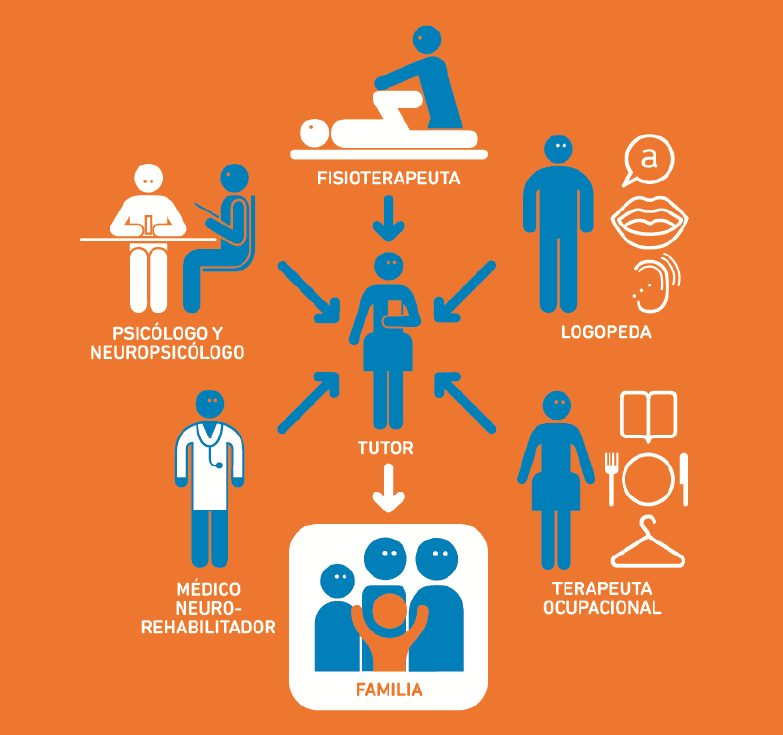
\includegraphics[scale=1.2]{neuroped}
    \caption{Equipo multidisciplinar - \textcopyright\ NeuroPed \cite{neuroped}}
    \label{neuropedimagen}
\end{figure}

Es por esto que pensamos que la universidad debería fomentar más el trabajo en equipo, fomentar la multidisciplinariedad y \textbf{eliminar las barreras} entre distintos campus de la universidad, y las numerosas trabas burocráticas que a veces nos encontramos para realizar proyectos así. Sin ir más lejos, este Trabajo de Fin de Grado ha requerido de un poco más de tiempo para poder llevarse a cabo esperando la aprobación de cada una de las facultades de los distintos integrantes del equipo.\\

Por ello, este equipo quiere promover el trabajo en equipo, construyendo un sistema que permita a las personas con grandes ideas, pero sin gente adecuada para llevarla a cabo, dar a conocer su proyecto y acercar a toda la universidad para que sea una realidad. Aunando los conceptos de \textit{``Smart City''} y Universidad, nace el nombre de \textbf{SmartU}, que engloba tanto al proyecto multidisciplinar como a las aplicaciones que vamos a crear.

\section{Objetivos}
\label{sec:objetivos}

Se pretende diseñar un sistema de información web que permita la \textbf{publicación de proyectos de carácter multidisciplinar} con el fin de promovermos entre la universidad y acercar más a las personas, no solo del ámbito universitario, sino también a las empresas y los ciudadanos ajenos al sistema educativo. Junto a éste, se creará también una aplicación móvil que acerce aun mas los contenidos expuestos en dicha plataforma web a las personas.\\

Estos son los principales objetivos que hemos planteado que deberían cumplirse a lo largo de la vida de este proyecto:

\begin{itemize}
    \item \textbf{Gestionar un equipo multidisciplinar:} Como forma de promover este tipo de equipos, el propio desarrollo se realizará sobre un equipo multidisciplinar, para analizar su progreso y detectar ventajas y fallos que deberían de subsanarse con el tiempo.
    \item \textbf{Creación de una metodología de trabajo multidisciplinar:} A lo largo del proyecto, se recopilará la información sobre cómo se ha trabajado, para así crear una especie de \textit{``Manual de trabajo de equipos multidisciplinares''}.
    \item \textbf{Creación de las plataformas software:} En el primer año de funcionamiento del proyecto, se quiere crear las primeras versiones de las plataformas web y móvil de creación y difusión de proyectos, como forma de demostrar el concepto sobre el que estamos trabajando y para comenzar a atraer la atención del público objetivo.
    \item \textbf{Marketing del proyecto:} Es importante crear una campaña de publicidad y difusión del proyecto que permita que la gente conozca lo que estamos haciendo, mostrando las ventajas que aportaría a la sociedad en general y el enriquecimiento que supondría para la docencia universitaria.
\end{itemize}

\subsection{Aplicación web}
Para la aplicación web me he planteado unos objetivos claros y simples:

\begin{itemize}
    \item La interfaz de usuario debe ser clara e intuitiva.
    \item La interfaz de usuario debe ser adaptable a todo tipo de tamaños de pantalla.
    \item La interfaz de usuario ha de ser lo menos intrusiva posible y dejar espacio a los contenidos relevantes.
    \item El código ha de ser claro y estar documentado de forma correcta para que otras personas puedan continuar y mejorar la aplicación.
\end{itemize}

En el siguiente apartado recojo algunas corrientes actuales de diseño y desarrollo, que me han servido para idear cómo debería ser la aplicación web que quiero crear, con el fin de que sea lo más usabe y útil posible para los usuarios.

\section{Estado del arte}
\subsection{Proyectos similares}
Como parte de la investigación realizada sobre este proyecto, encontramos algunas plataformas con una idea subyacente similar a la que estamos trabajando: prima la colaboración en equipo, el acercamiento de sectores de la sociedad y la creación de proyectos.

\begin{itemize}
    \item \textbf{Medialab UGR} \cite{medialabugr} se concibe como un espacio de encuentro para el análisis, investigación y difusión de las posibilidades que las tecnologías digitales generan en la cultura y en la sociedad en general.
    \item \textbf{Link by UMA-ATech} \cite{linkuma} reúne a asociaciones, estudiantes, empresas, emprendedores y todo tipo de expertos para compartir ideas, aprender y crecer juntos. En definitiva, Link es un espacio para crear grandes proyectos.
    \item \textbf{LinkedIn} \cite{linkedin} es una comunidad social orientada a las empresas, a los negocios y el empleo. Partiendo del perfil de cada usuario, que libremente revela su experiencia laboral y sus destrezas en un verdadero currículum laboral, la web pone en contacto a millones de empresas y empleados.
    \item \textbf{Kickstarter} \cite{kickstarter} es un sitio web de micromecenazgo en el que los usuarios pueden publicar sus proyectos y obtener financiación de la gente para poder llevarlo a cabo. En caso de que el proyecto haya tenido éxito financiándose, los donantes reciben recompensas relacionadas con el proyecto que se va a realizar.
\end{itemize}

\subsection{Usabilidad y UX}
En el campo de la usabilidad y la \textit{User Experience} (UX) se ha dicho mucho con el objetivo de encontrar la clave de un sistema que sea usable y amigable para todos los grupos de usuarios de tecnología que existen actualmente. Se hace necesario para lograr éxito que las interfaces sean sencillas de entender y claras, con una estructura que no haga que el usuario desinstale la aplicación o cierre la pestaña del navegador.\\

Por ello, para este proyecto he decidido construir mi aplicación web en base a unos principios de diseño actuales y que siguen creciendo con el paso del tiempo.

\subsubsection{Diseño adaptable o \textit{responsive}}
El diseño adaptable establece que un sistema informático (ya sea una página web, un programa de ordenador o una aplicación móvil) debe ser \textbf{reactivo} a la interacción del usuario con el mismo y al entorno en el que se encuentra. Esto quiere decir que ha de ``adaptarse'' a todo tipo de dispositivos donde se esté ejecutando o visualizando.\\

Ya sea en una pantalla de 24 pulgadas, o un smartphone de 5, el sistema ha de ser capaz de mostrar la misma información y de proporcionar la misma funcionalidad, \textbf{reorganizando los contenidos} de la interfaz para que nada quede inaccesible. En la figura \ref{water} podemos ver de forma gráfica el concepto que aquí se expone.\\

En este sentido, existe un framework de diseño adaptable que nos facilita la tarea de crear un sistema usable en todo tipo de formatos de pantalla, \textbf{Bootstrap} \cite{bootstrap}. Proporciona un conjunto de elementos para el \textit{``layout''} de la aplicación y objetos de interacción como pestañas, botones, paneles, etc.

\begin{figure}
    \centering
    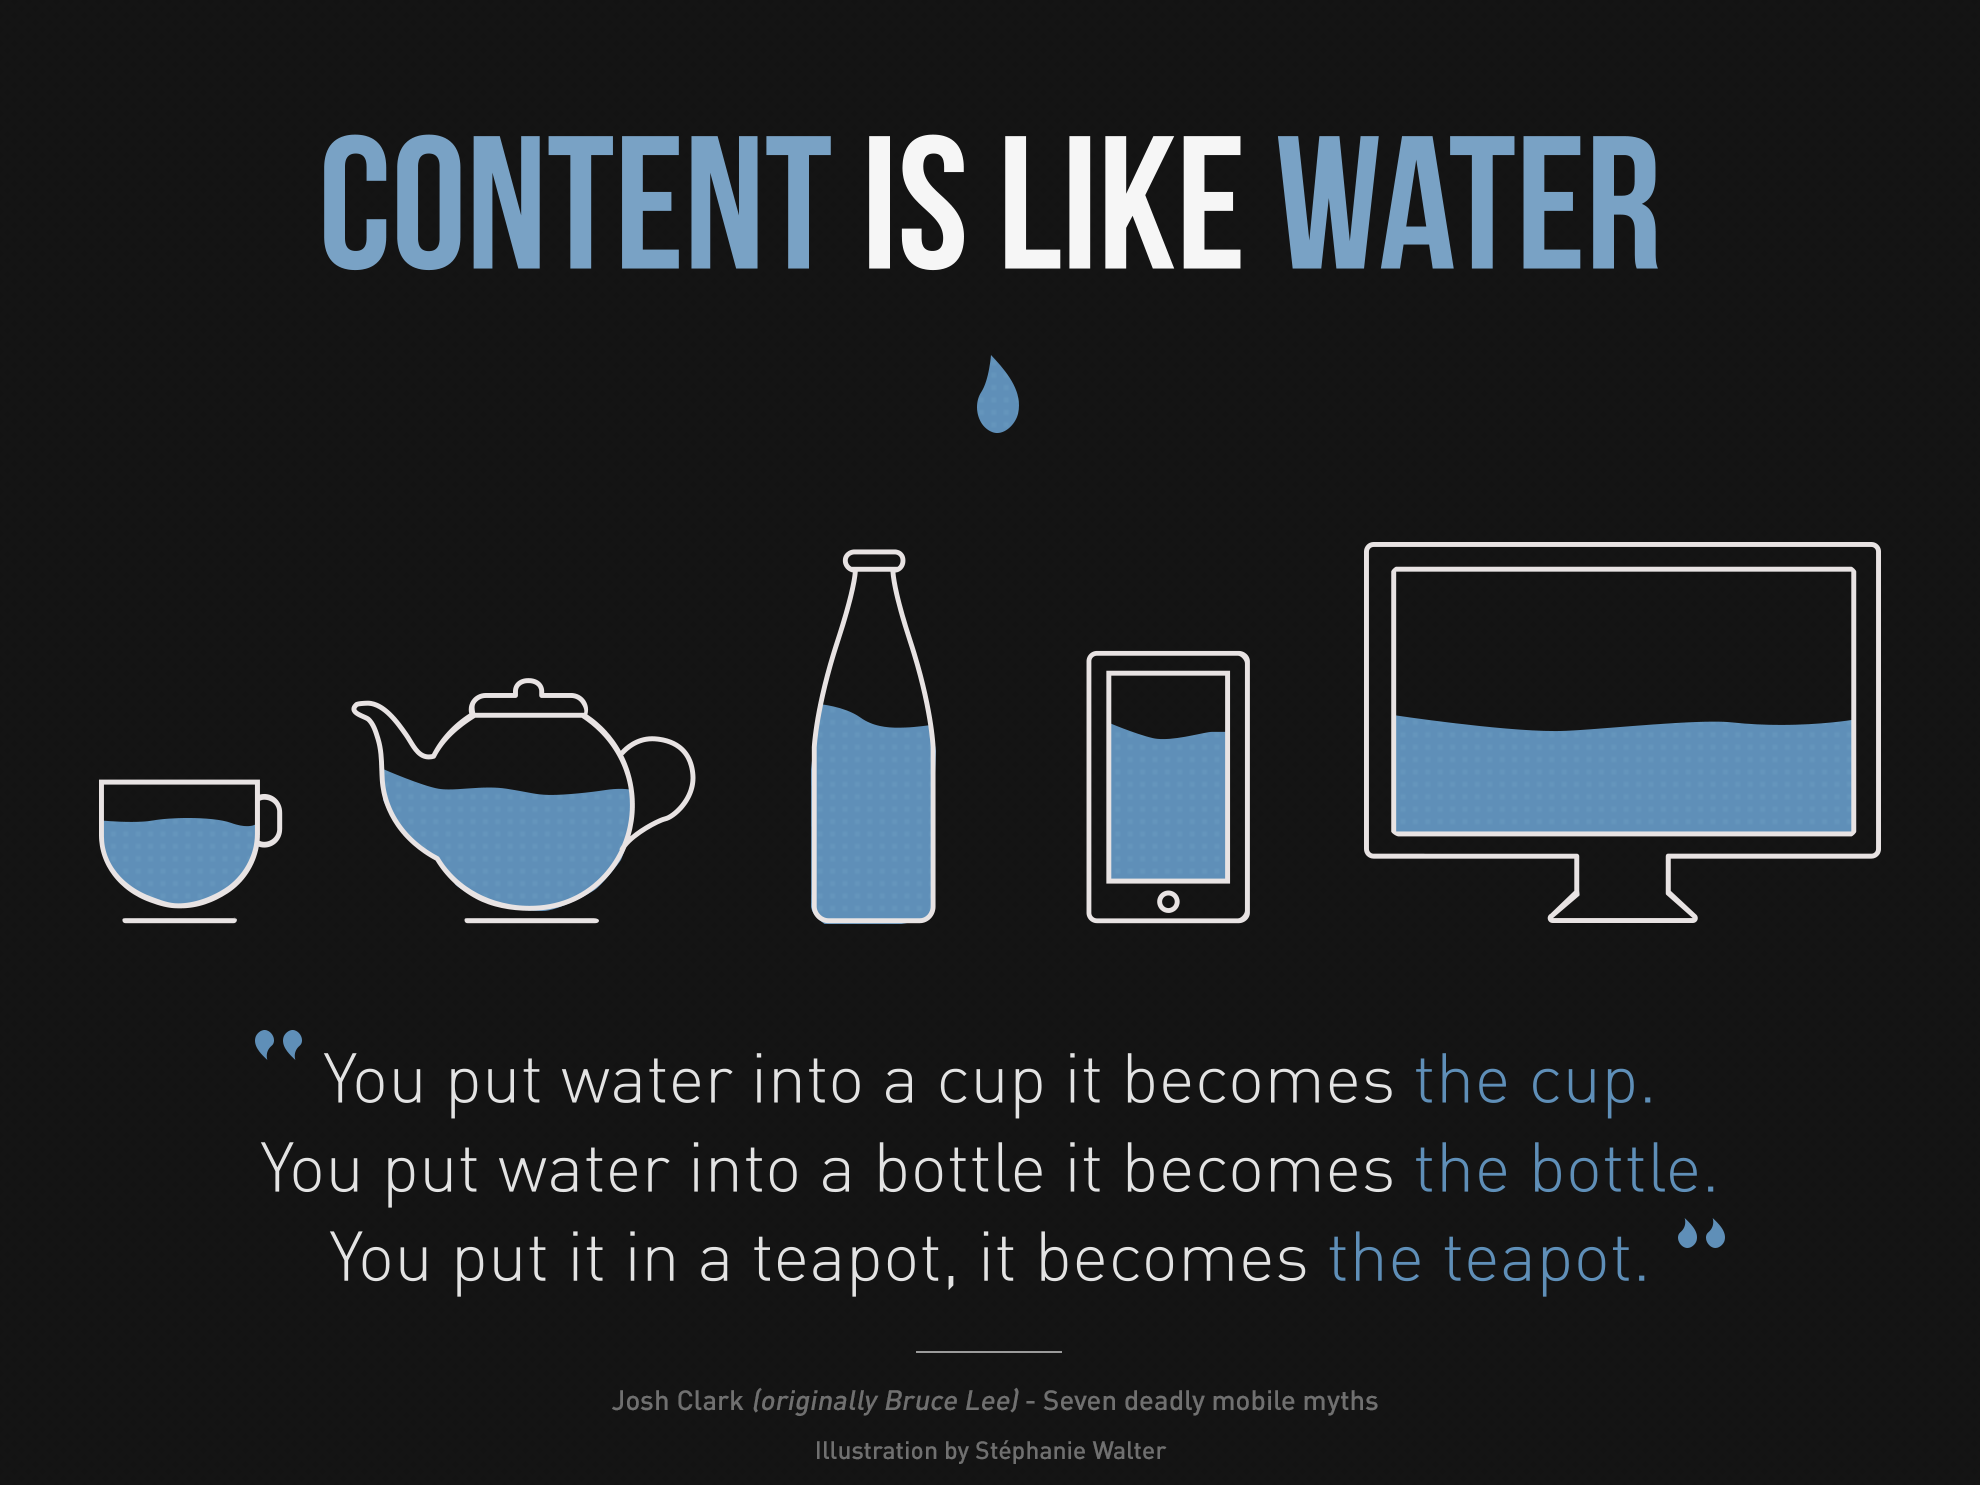
\includegraphics[scale=0.165]{water}
    \caption{\textit{``El contenido es como el agua''} - \textcopyright\ Clark y Walter \cite{contentwater}}
    \label{water}
\end{figure}

\section{Estructura de este documento}
Esperando que este primer capítulo haya despertado tu interés, quiero detallar, a modo de resumen, qué es lo que vas a encontrarte a continuación:

\begin{itemize}
    \item En el \textit{capítulo \ref{ch:metodologia}} (\textbf{Metodología}), hablo de la forma de trabajar que hemos seguido para llevar a cabo el proyecto, los integrantes que han compuesto el equipo, el trabajo realizado por cada uno de ellos (detallando principalmente el que yo he realizado), cómo se han gestionado las cosas y los resultados que se han obtenido de dicha colaboración.
    \item En el \textit{capítulo \ref{ch:desarrollo}} (\textbf{Desarrollo}), se abarca el desarrollo del producto, es decir, la aplicación web de SmartU para la publicación de proyectos y difusión de opiniones e ideas. Se estructura en diversos apartados siguiendo la estructura típica del proceso de desarrollo de software.
    \item En el \textit{capítulo \ref{ch:descripcion}} (\textbf{Descripción}), se muestra la aplicación web creada, describiendo sus características y su interfaz de usuario. También vienen incluidas unas instrucciones para instalar la aplicación en nuestros propios equipos y probar su funcionalidad en persona.
    \item En el \textit{capítulo \ref{ch:conclusiones}} (\textbf{Conclusiones}), dedico unas palabras para hacer balance y análisis de cómo ha sido la experiencia trabajando en este proyecto, así como una propuesta de mejoras para el futuro que se podrían aplicar.
    \item En el \textit{capítulo \ref{ch:anexos}} (\textbf{Anexos}), se incluyen materiales adicionales que complementan la información de algunos de los capítulos de esta documentación.
\end{itemize}
